\documentclass[10pt,xcolor=pdflatex]{beamer}
\usepackage{newcent}
\usepackage[utf8]{inputenc}
\usepackage[czech]{babel}
\usepackage{hyperref}
\usepackage{fancyvrb}
\usetheme{FIT}

%%%%%%%%%%%%%%%%%%%%%%%%%%%%%%%%%%%%%%%%%%%%%%%%%%%%%%%%%%%%%%%%%%
\title[Bakalářská práce]{Android aplikace pro Git s podporou git-lfs a git-annex}

\author[]{Petr Marek}

\institute[]{Fakulta informačních technologií VUT v Brně\\
Bo\v{z}et\v{e}chova 1/2. 612 66 Brno - Kr\'alovo Pole\\}

%\date{January 1, 2016}
%\date{\today}
\date{} % bez data

%%%%%%%%%%%%%%%%%%%%%%%%%%%%%%%%%%%%%%%%%%%%%%%%%%%%%%%%%%%%%%%%%%

\begin{document}

\frame[plain]{\titlepage}

\begin{frame}\frametitle{Cíl práce}
    \begin{itemize}
        \item{Git, git-lfs a git-annex}
        \item{Uživatelsky přívětivé rozhraní}
        \item{Minimalizace velikosti repozitářů}
        \item{Rozšiřitelnost}
    \end{itemize}
\end{frame}

\begin{frame}\frametitle{Návrh aplikace}
    \begin{columns}
        \column{0.5\textwidth}
            \begin{itemize}
                \item{Architektura}
                \item{Integrace Gitu}
                \item{Uživatelské rozhraní}
            \end{itemize}
        \column{0.4\textwidth}
            \frame{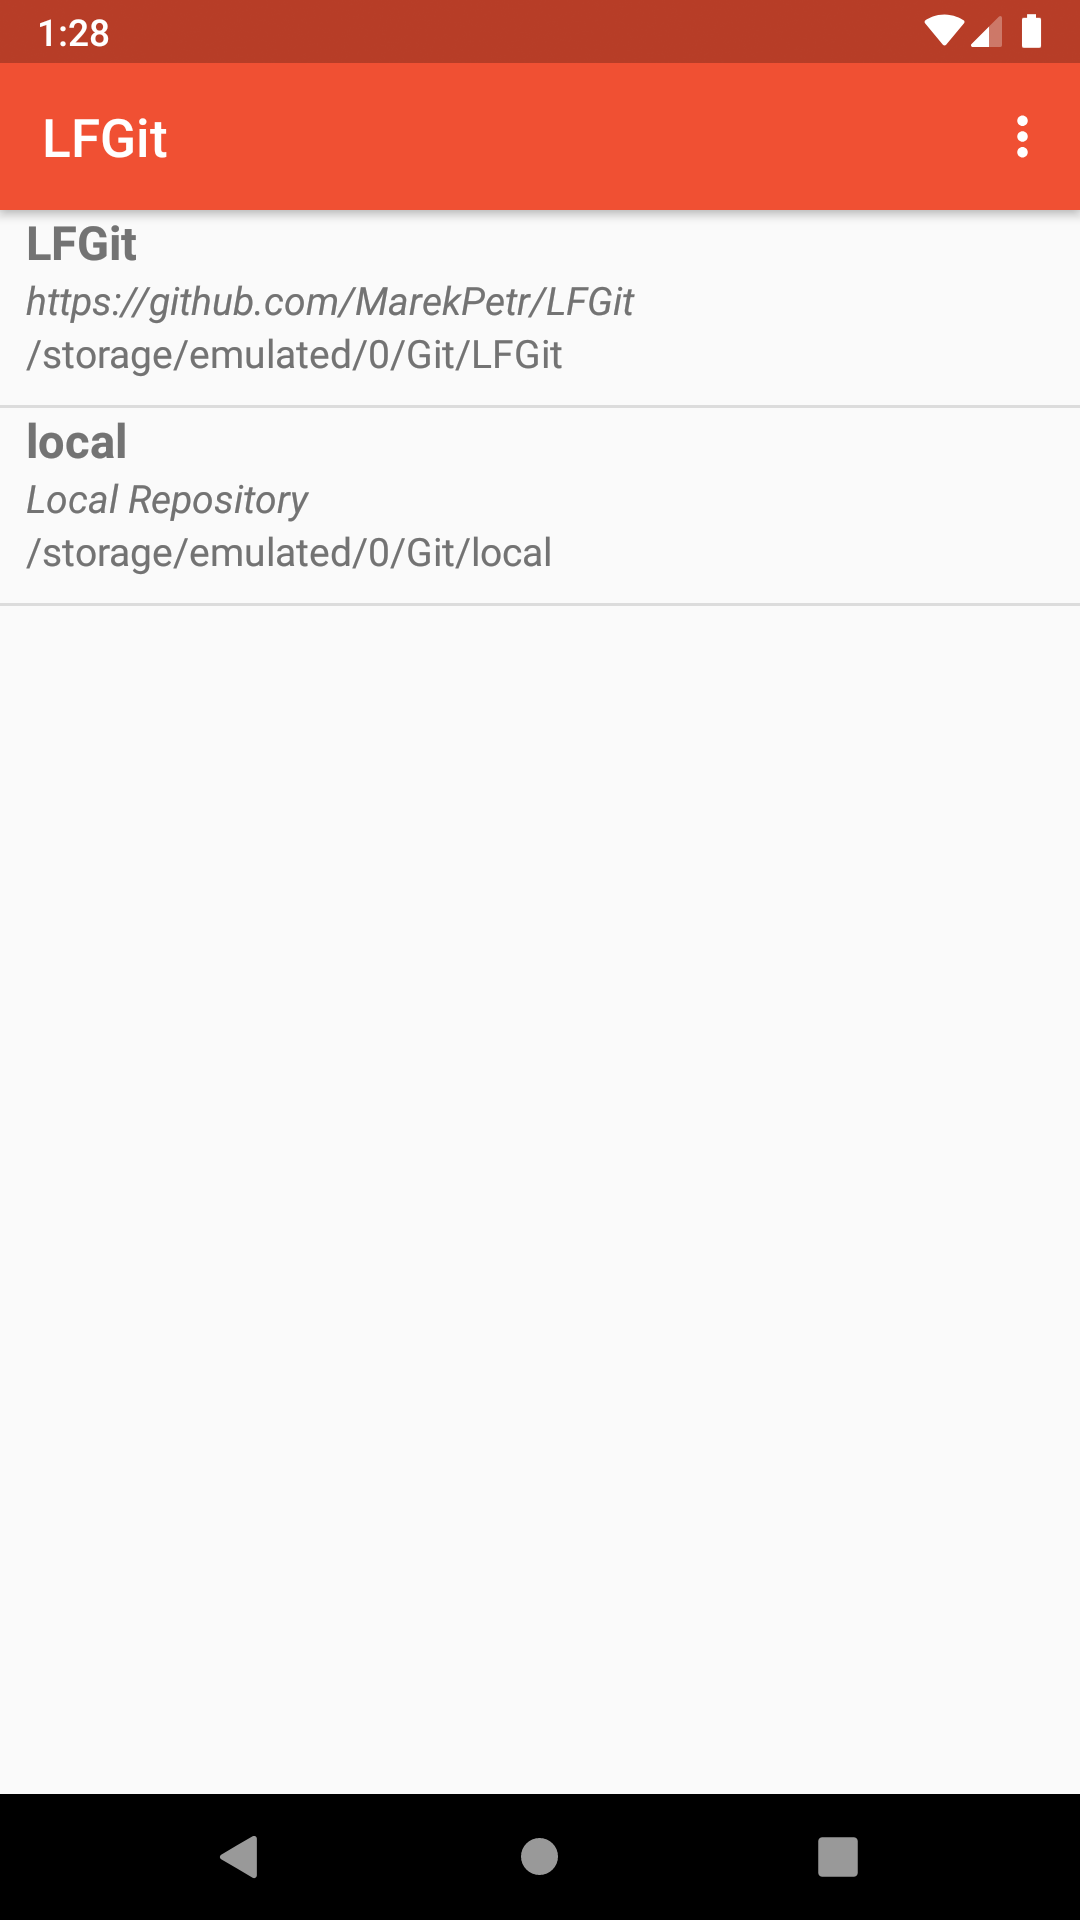
\includegraphics[scale=0.08]{img/repo_list}}
    \end{columns}
\end{frame}

\begin{frame}\frametitle{Výsledky}
    \begin{columns}
        \column{0.5\textwidth}
            \begin{itemize}
                \item {Funkcionalita}
                \item {Srovnání s konkurencí}
                \item {Možná rozšíření}
            \end{itemize}
        \column{0.4\textwidth}
            \frame{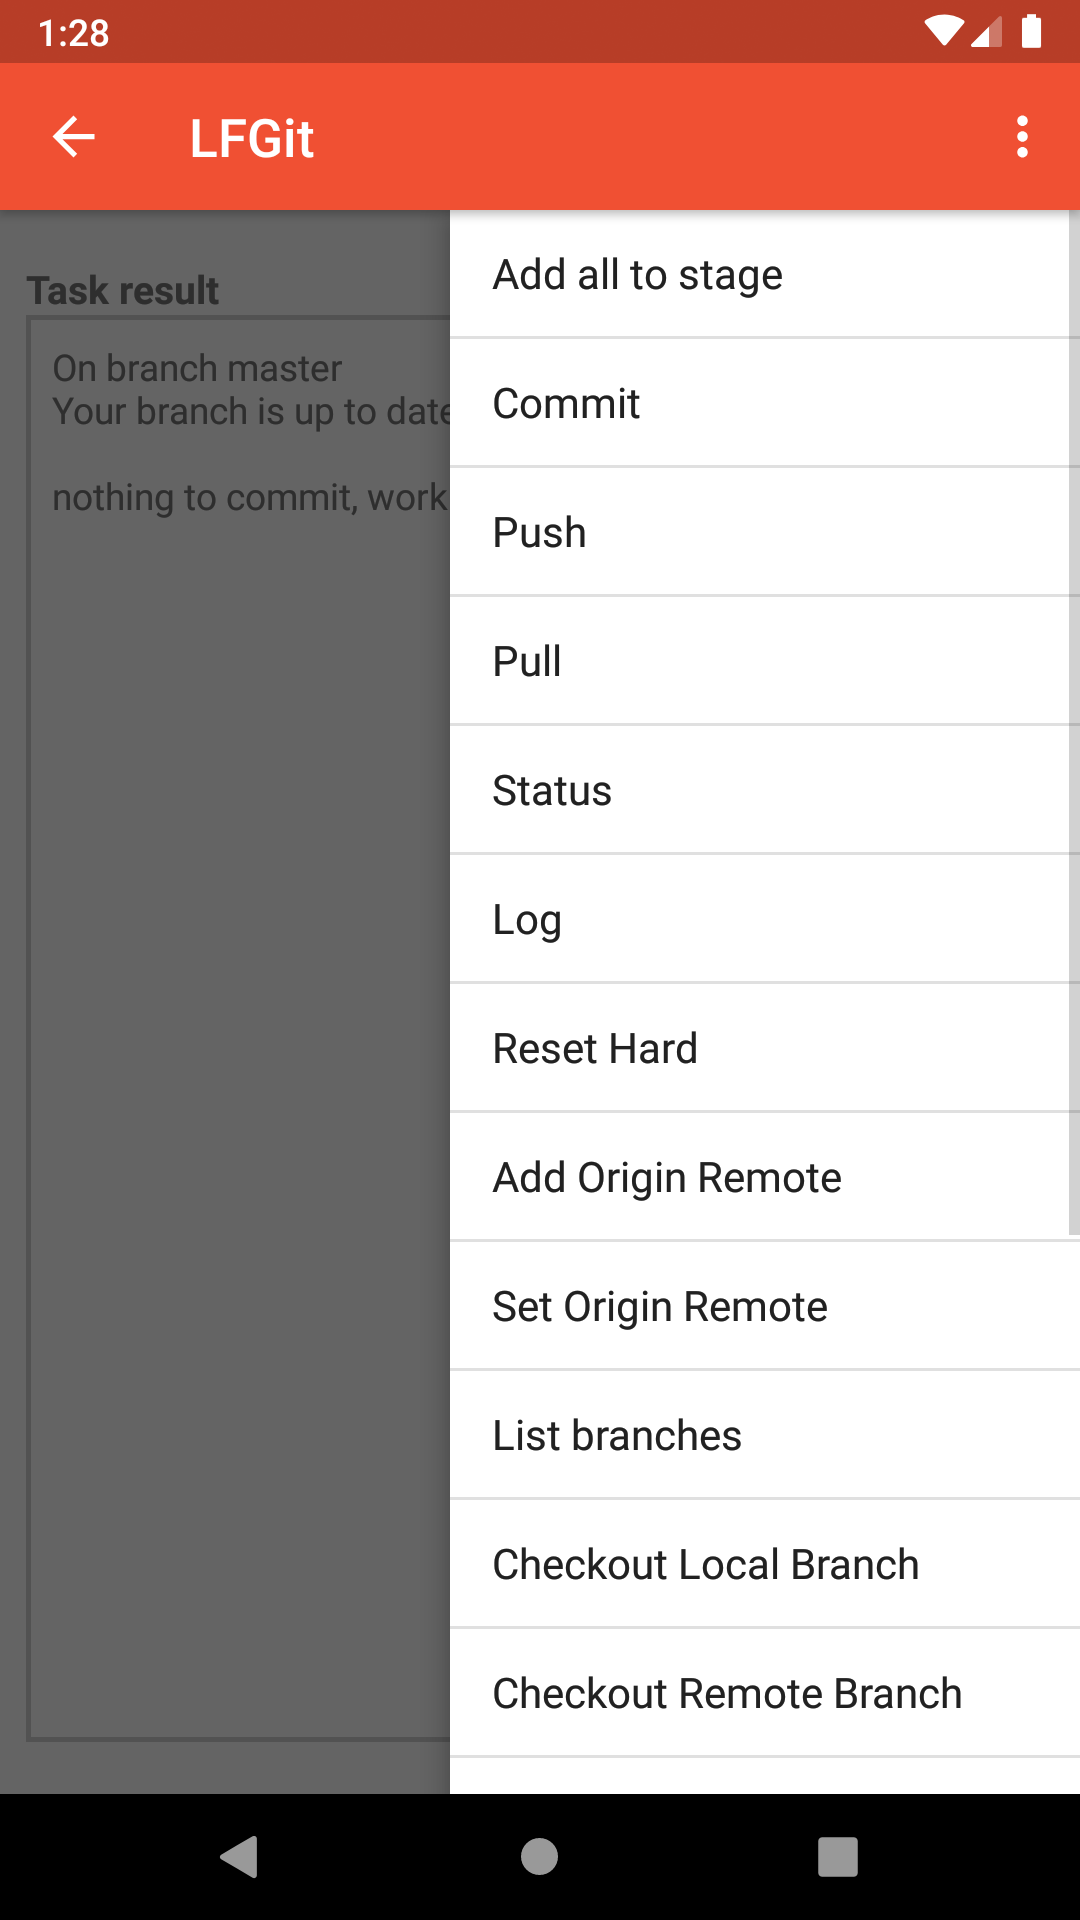
\includegraphics[scale=0.08]{img/tasks}}
    \end{columns}
\end{frame}

\begin{frame}\frametitle{Diskuze}
    \begin{columns}
        \column{0.5\textwidth}
            \begin{itemize}
            \item{Role údajů v databázi}
            \item{Docker a termux-packages}
            \item{Další otázky...}            \end{itemize}
        \column{0.4\textwidth}
            \vspace{0.7cm}
            \begin{figure}[b]
                \frame{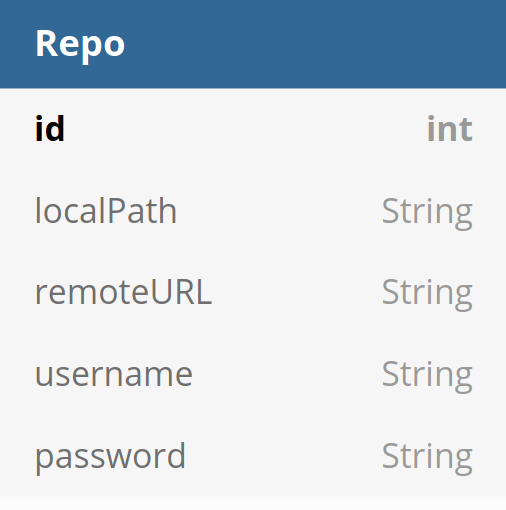
\includegraphics[scale=0.15]{img/repo}}
            \end{figure}
    \end{columns}
\end{frame}
\end{document}
